\section{Unit Test và Báo cáo JaCoCo}
\label{sec:unittest}

\newcommand{\jacocofigureplaceholder}[3]{
\begin{figure}[H]
    \centering
    \IfFileExists{#1}{
        \includegraphics[width=0.92\textwidth]{#1}
    }{
        \fbox{
            \parbox[c][0.22\textheight][c]{0.86\textwidth}{
                \centering
                Ảnh JaCoCo Coverage cho module \texttt{#2}\\
                \texttt{#1}
            }
        }
    }
    \caption{#3}
\end{figure}
}

\subsection{Hướng dẫn chung chạy Unit Test}
Dự án YAS sử dụng cấu trúc monorepo Maven. Khi cần chạy test cho một service cụ thể, lệnh được thực thi từ thư mục gốc repository và truyền tên module qua tham số \texttt{-pl}. Sau khi test hoàn tất, JaCoCo sinh báo cáo tại \texttt{<module>/target/site/jacoco/index.html}.

\begin{lstlisting}[language=bash, caption={Lệnh chạy test và sinh báo cáo JaCoCo cho từng module}]
./mvnw -f pom.xml test -pl <module> -am
./mvnw -f pom.xml test jacoco:report -pl <module> -am
open <module>/target/site/jacoco/index.html
\end{lstlisting}

Quy trình trên được dùng để kiểm tra độc lập từng service trước khi đẩy Pull Request. Pipeline Jenkins cũng chạy test theo module thay đổi, upload JUnit report và xuất JaCoCo report để phục vụ bước kiểm tra coverage.

\subsection{Chi tiết Unit Test theo Service}
Tương tự format phần Unit Test của báo cáo tham khảo, mỗi service được trình bày thống nhất bằng kết quả chạy unit test và ảnh JaCoCo tương ứng. Phần này không lặp lại thông tin triển khai hoặc số liệu chi tiết vì các thông tin này đã nằm trong lịch sử Pull Request, Jenkins và JaCoCo.

\subsubsection{Module media}
\textbf{Kết quả:} Unit test chạy thành công và báo cáo JaCoCo được sinh để phục vụ kiểm tra coverage.

\jacocofigureplaceholder{img/media.png}{media}{Báo cáo JaCoCo Coverage -- module media}

\subsubsection{Module product}
\textbf{Kết quả:} Unit test chạy thành công và báo cáo JaCoCo được sinh để phục vụ kiểm tra coverage.

\jacocofigureplaceholder{img/product.png}{product}{Báo cáo JaCoCo Coverage -- module product}

\subsubsection{Module order}
\textbf{Kết quả:} Unit test chạy thành công và báo cáo JaCoCo được sinh để phục vụ kiểm tra coverage.

\jacocofigureplaceholder{img/order.png}{order}{Báo cáo JaCoCo Coverage -- module order}

\subsubsection{Module inventory}
\textbf{Kết quả:} Unit test chạy thành công và báo cáo JaCoCo được sinh để phục vụ kiểm tra coverage.

\jacocofigureplaceholder{img/inventory.png}{inventory}{Báo cáo JaCoCo Coverage -- module inventory}

\subsubsection{Module payment}
\textbf{Kết quả:} Unit test chạy thành công và báo cáo JaCoCo được sinh để phục vụ kiểm tra coverage.

\jacocofigureplaceholder{img/payment.png}{payment}{Báo cáo JaCoCo Coverage -- module payment}

\subsubsection{Module payment-paypal}
\textbf{Kết quả:} Unit test chạy thành công và báo cáo JaCoCo được sinh để phục vụ kiểm tra coverage.

\jacocofigureplaceholder{img/payment-paypal.png}{payment-paypal}{Báo cáo JaCoCo Coverage -- module payment-paypal}

\subsubsection{Module promotion}
\textbf{Kết quả:} Unit test chạy thành công và báo cáo JaCoCo được sinh để phục vụ kiểm tra coverage.

\jacocofigureplaceholder{img/promotion.png}{promotion}{Báo cáo JaCoCo Coverage -- module promotion}

\subsubsection{Module rating}
\textbf{Kết quả:} Unit test chạy thành công và báo cáo JaCoCo được sinh để phục vụ kiểm tra coverage.

\jacocofigureplaceholder{img/rating.png}{rating}{Báo cáo JaCoCo Coverage -- module rating}

\subsubsection{Module delivery}
\textbf{Kết quả:} Unit test chạy thành công và báo cáo JaCoCo được sinh để phục vụ kiểm tra coverage.

\jacocofigureplaceholder{img/delivery.png}{delivery}{Báo cáo JaCoCo Coverage -- module delivery}

\subsubsection{Module recommendation}
\textbf{Kết quả:} Unit test chạy thành công và báo cáo JaCoCo được sinh để phục vụ kiểm tra coverage.

\jacocofigureplaceholder{img/recommendation.png}{recommendation}{Báo cáo JaCoCo Coverage -- module recommendation}

\subsubsection{Module customer}
\textbf{Kết quả:} Unit test chạy thành công và báo cáo JaCoCo được sinh để phục vụ kiểm tra coverage.

\jacocofigureplaceholder{img/customer.png}{customer}{Báo cáo JaCoCo Coverage -- module customer}

\subsubsection{Module location}
\textbf{Kết quả:} Unit test chạy thành công và báo cáo JaCoCo được sinh để phục vụ kiểm tra coverage.

\jacocofigureplaceholder{img/location.png}{location}{Báo cáo JaCoCo Coverage -- module location}

\subsubsection{Module cart}
\textbf{Kết quả:} Unit test chạy thành công và báo cáo JaCoCo được sinh để phục vụ kiểm tra coverage.

\jacocofigureplaceholder{img/cart.png}{cart}{Báo cáo JaCoCo Coverage -- module cart}

\subsubsection{Module tax}
\textbf{Kết quả:} Unit test chạy thành công và báo cáo JaCoCo được sinh để phục vụ kiểm tra coverage.

\jacocofigureplaceholder{img/tax.png}{tax}{Báo cáo JaCoCo Coverage -- module tax}

\subsubsection{Module webhook}
\textbf{Kết quả:} Unit test chạy thành công và báo cáo JaCoCo được sinh để phục vụ kiểm tra coverage.

\jacocofigureplaceholder{img/webhook.png}{webhook}{Báo cáo JaCoCo Coverage -- module webhook}

\subsection{Coverage Gate trong Jenkins}
Coverage Gate được đặt tại pipeline để bảo đảm mỗi PR không chỉ chạy pass unit test mà còn tạo được báo cáo độ phủ. Script \texttt{ci/check-coverage.sh} đọc chỉ số LINE coverage từ file \texttt{jacoco.xml} của module và so sánh với ngưỡng cấu hình.

\begin{lstlisting}[language=bash, caption={check-coverage.sh -- kiểm tra ngưỡng coverage}]
module="$1"
minimum="$2"
report_path="${module}/target/site/jacoco/jacoco.xml"

line_counter="$(grep '<counter type="LINE"' "${report_path}" | tail -1)"
covered="$(echo "${line_counter}" | sed 's/.*covered="\([0-9]*\)".*/\1/')"
missed="$(echo "${line_counter}" | sed 's/.*missed="\([0-9]*\)".*/\1/')"

total=$((covered + missed))
coverage_percent="$(awk -v c="${covered}" -v t="${total}" \
    'BEGIN { printf "%.2f", (c / t) * 100 }')"

awk -v actual="${coverage_percent}" -v threshold="${minimum}" \
    'BEGIN { exit !(actual + 0 >= threshold + 0) }'
\end{lstlisting}

\begin{itemize}[noitemsep]
    \item \textbf{Ngưỡng kiểm tra}: cấu hình qua biến \texttt{COVERAGE\_THRESHOLD}.
    \item \textbf{Mức đọc dữ liệu}: dùng counter \texttt{LINE} cấp report-level trong \texttt{jacoco.xml}.
    \item \textbf{Tích hợp Jenkins}: nếu coverage thấp hơn ngưỡng, stage Coverage Gate trả lỗi và pipeline thất bại.
    \item \textbf{Minh chứng}: console log Jenkins hiển thị module được kiểm tra, phần trăm coverage thực tế và kết quả pass/fail.
\end{itemize}

\begin{figure}[H]
    \centering
    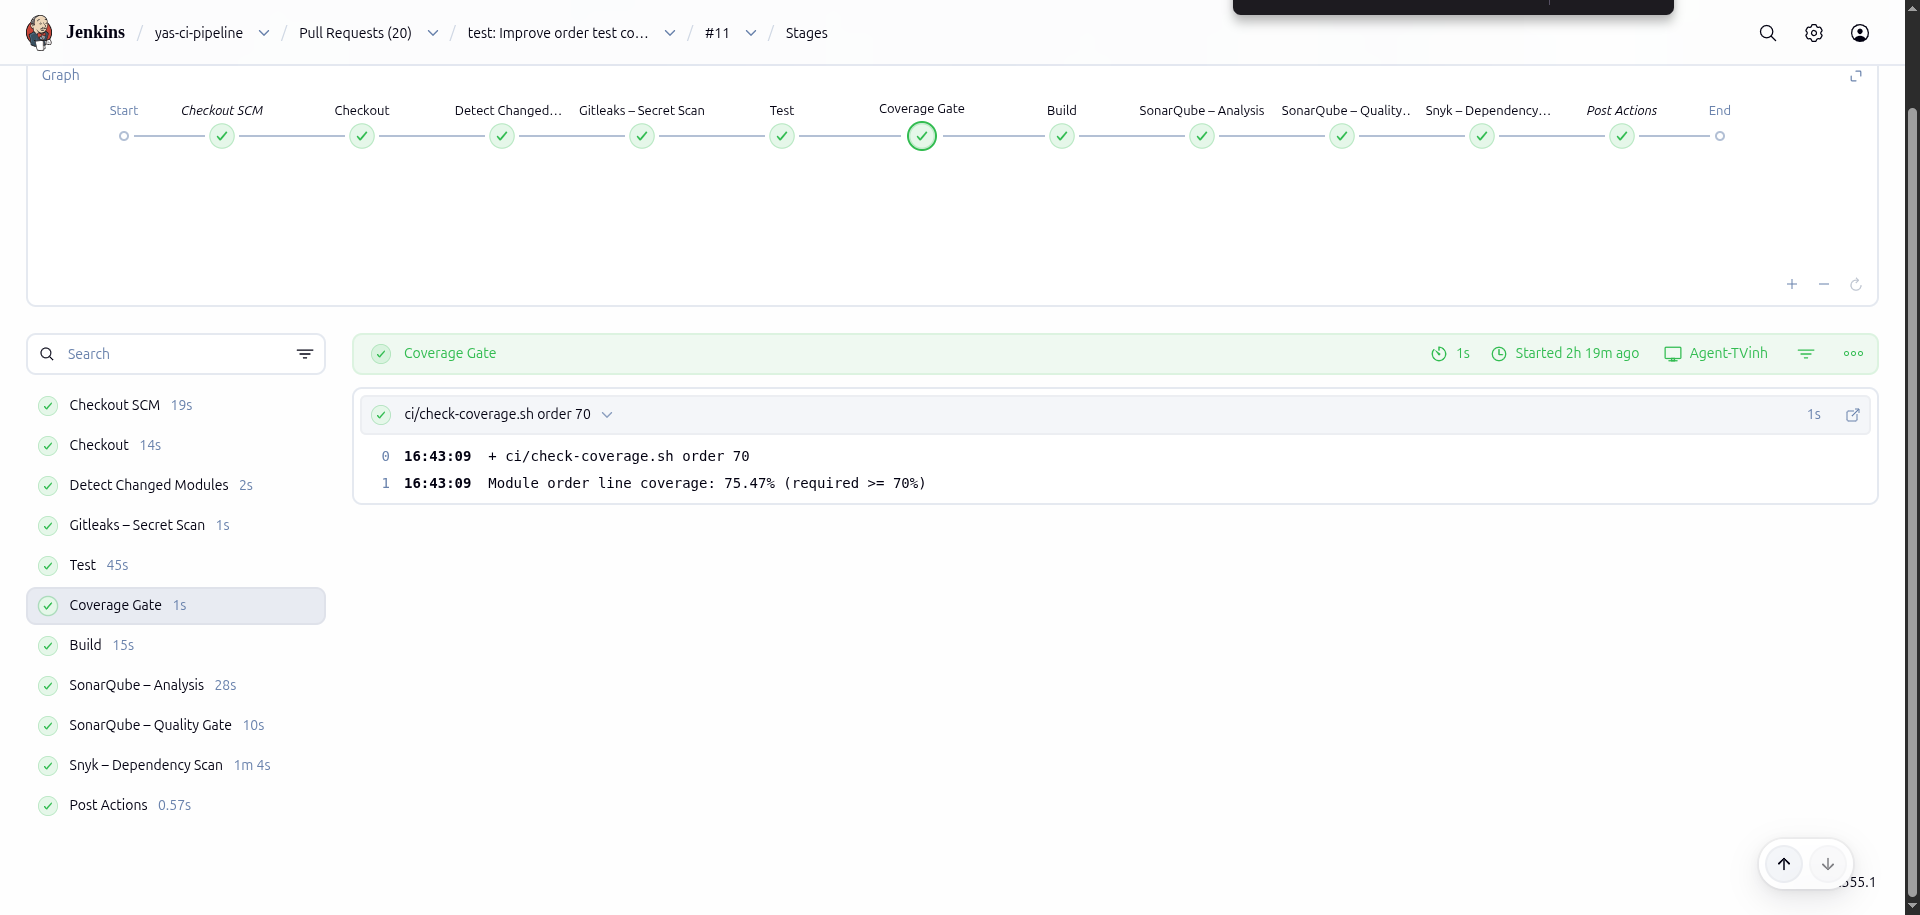
\includegraphics[width=0.92\textwidth]{img/10-jenkins-console-coverage-gate.png}
    \caption{Console output Jenkins khi kiểm tra ngưỡng Coverage Gate}
\end{figure}
